%%%%%%%%%%%%%%%%%%%%%%%%%%%%%
%% Styles, packages and new commands
\input{../../Main/ML_Main.tex}
%%%%%%%%%%%%%%%%%%%%%%%%%%%%%
%% Edit the title page
\title{Machine Learning}
\subtitle{Module 3.1 - Models: Linear and Logistic regressions}
\author[MOB]{Marc-Olivier Boldi}
\institute[HEC MSc Mgt BA]{Master in Management, Business Analytics, HEC UNIL}
\date[Spring 2024]{Spring 2024}
%%%%%%%%%%%%%%%%%%%%%%%%%%%%%
%%%%%%%%%%%%%%%%%%%%%%%%%%%%%
%%%%%%%%%%%%%%%%%%%%%%%%%%%%%
%%%%%%%%%%%%%%%%%%%%%%%%%%%%%
\begin{document}
%%%%%%%%%%%%%%%%%%%%%%%%%%%%%
\begin{frame}
  \titlepage
\end{frame}
%%%%%%%%%%%%%%%%%%%%%%%%%%%%%
\begin{frame}
\frametitle{Table of Contents}
	\tableofcontents
\end{frame}
%%%%%%%%%%%%%%%%%%%%%%%%%%%%%
\section{Linear regression}
%%%%%%%%%%%%%%%%%%%%%%%%%%%%%
\begin{frame}
\frametitle{Linear regression}
The prediction formula is 
$$
f(x;\theta) = \theta_0 + \theta_1 x_{1} + \ldots + \theta_p x_{p}
$$
\begin{center}
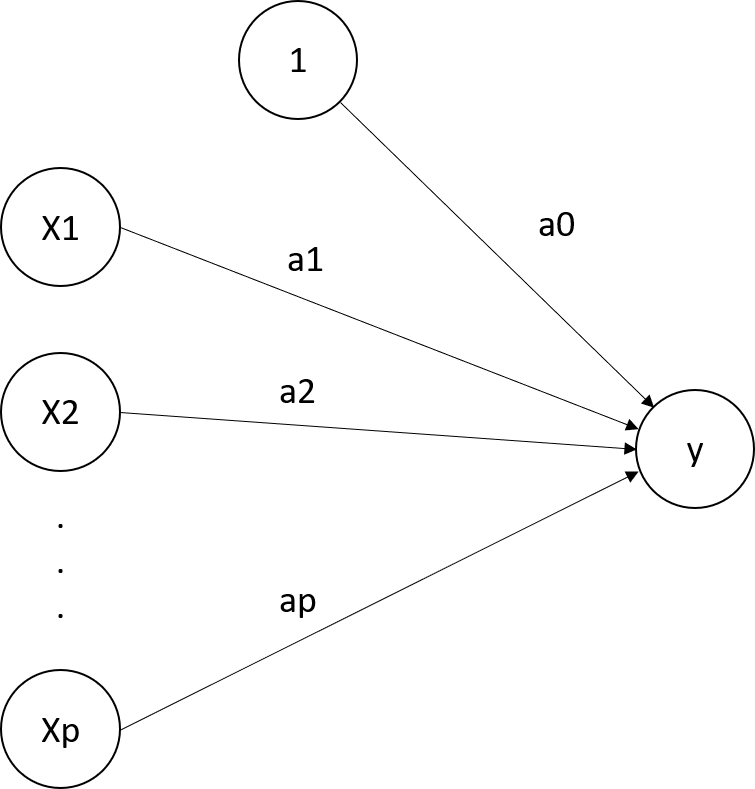
\includegraphics[width=4cm]{../../Graphs/LinReg_Network.png}
\end{center}
\end{frame}
%%%%%%%%%%%%%%%%%%%%%%%%%%%%%
\begin{frame}
\frametitle{The MSE and the OLS}
The loss function is the {\bf mean squared error}, MSE,
$$
\bar{\cal L}(\theta) = \frac{1}{n} \sum_{i=1}^n \{y_i - f(x_i;\theta)\}^2.
$$
The optimal parameter under this loss is called the {\bf Ordinary Least Squares}, OLS,
$$
\hat{\theta} = \arg\min_{\theta} \frac{1}{n} \sum_{i=1}^n \{y_i - f(x_i;\theta)\}^2.
$$
\end{frame}
%%%%%%%%%%%%%%%%%%%%%%%%%%%%%
\begin{frame}
\frametitle{The OLS}
To find the OLS, the algorithm is exact and the final solution can be explicitly computed with the matrix-operation
$$
\hat{\theta} = (X^TX)^{-1} X^T y,
$$ 
where
\begin{itemize}
\item $X$ is the so-called {\bf design matrix} of size $n\times (p+1)$ and whose $i$-th row contains 
$$
[1,x_{i1},\ldots,x_{ip}],
$$
\item $y$ is the vector of length $n$ whose $i$-th element is $y_i$.
\end{itemize}
\end{frame}
%%%%%%%%%%%%%%%%%%%%%%%%%%%%%
\section{Logistic regression}
%%%%%%%%%%%%%%%%%%%%%%%%%%%%%
\begin{frame}
\frametitle{Logistic regression}
The logistic regression is a model for {\bf binary classification}. Prediction formula is in several steps:
\begin{itemize}
\item Compute the {\bf linear predictor}
$$
z(x;\theta) = \theta_0 + \theta_1 x_{1} + \cdots + \theta_p x_{p},
$$
\item Compute the {\bf probability prediction} (sigmoid function):
$$
p(x;\theta) = P(Y=1 | X=x) = \frac{\exp\{z(x;\theta)\}}{1+\exp\{z(x;\theta)\}}.
$$
\item Compute the {\bf prediction of the class}: 
$$
f(x;\theta) = \left\{
\begin{array}{ll}
1, & \mbox{if } p\geq 0.5,\\
0, & \mbox{if } p < 0.5.
\end{array}
\right.
$$
\end{itemize}
\end{frame}
%%%%%%%%%%%%%%%%%%%%%%%%%%%%%
\begin{frame}
\frametitle{The sigmoid and the logit function}
The {\bf logit function} is the inverse of the {\bf sigmoid function} and thus transforms $p(x;\theta)$ to $z(x;\theta)$.
$$
z(x;\theta) = \log \frac{p(x;\theta)}{1-p(x;\theta)}
$$ 
\end{frame}
%%%%%%%%%%%%%%%%%%%%%%%%%%%%%
\begin{frame}
\frametitle{Estimation}
The loss function uses the probabilities $p(x;\theta)$ and not the final predictions. The loss is the {\bf cross-entropy} also called {\bf negative log-likelihood}:
$$
{\cal L}(y,p) = -y \log p - (1-y) \log (1-p).
$$
Interpretation,
\begin{itemize}
\item If $y=1$, we want $p$ to be large (close to 1). The loss is 
$$
{\cal L}(1,p) = - \log p
$$
It will be small indeed if $p$ is large.
\item If $y=0$, we want $p$ to be small (close to 0). The loss is
$$
{\cal L}(0,p) = - \log (1-p)
$$
It will be small indeed if $p$ is small.
\end{itemize}
\end{frame}
%%%%%%%%%%%%%%%%%%%%%%%%%%%%%
\begin{frame}
\frametitle{Estimation}
The overall loss is
$$
\bar{{\cal L}}(\theta) = -\frac{1}{n} \sum_{i=1}^n y_i \log p(x_i;\theta) + (1-y_i) \log \{1-p(x_i;\theta)\}.
$$
The $\log$ in this formula can be in any base. Often,
\begin{itemize}
\item Machine learners use $\log_2$,
\item Statisticians use $\ln$.
\end{itemize}
This has absolutely no consequence on the final result (all $\log$ are equivalent here). But it can bring confusion from time to time.
\end{frame}
%%%%%%%%%%%%%%%%%%%%%%%%%%%%%
\begin{frame}
\frametitle{Optimal parameters}
To obtain the optimal parameters, the best algorithm is the {\bf Newton-Raphson} algorithm. It requires 
\begin{itemize}
\item To compute the first and second derivatives of $\bar{\cal L}(\theta)$,
\item To build a sequence of $\hat{\theta}_k$ that converges to the optimal one using these derivatives. 
\end{itemize}
This algorithm is very fast and efficient. However, there is no explicit formula for $\hat{\theta}$, unlike the OLS.\\
\vspace{0.3cm}
The optimal $\hat{\theta}$ is sometimes called the {\bf maximum likelihood estimator}, {\bf MLE}. That terminology is however less usual among machine learners than statisticians.
\end{frame}
%%%%%%%%%%%%%%%%%%%%%%%%%%%%%
\section{Interpretation}
%%%%%%%%%%%%%%%%%%%%%%%%%%%%%
\begin{frame}
\frametitle{Interpretation}
Linear and logistic regressions are highly interpretable in that 
\begin{itemize}
\item the coefficients quantify the link between the features $x$ and the outcome $y$.
\item the certainty of the prediction can be quantify.
\end{itemize}
\end{frame}
%%%%%%%%%%%%%%%%%%%%%%%%%%%%%
\begin{frame}
\frametitle{Interpretation of the coefficients}
For the {\bf linear regression}, coefficients are interpreted as {\it slopes}.
\begin{itemize}
\item When the feature $x_1$ increases by $1$ unit, the outcome $y$ increases in average by $\theta_1$ units (same for all features $1,\ldots,p$).
\item A positive coefficient $\theta_j$ means a positive linear association between the feature $x_j$ and the outcome $y$.
\item The larger the coefficients, the larger the association, in absolute value. (note: pay attention to the scale!)
\item For the categorical features, the coefficients estimate the average change in the outcome $y$ when the feature switches from the reference level to any other level. It is thus a {\bf contrast} with the reference level.  
\end{itemize}
\small
Note: one should not say that an increase in $x_j$ {\it causes} an increase of the response. It is an association. The causality implies a direction and is more complex to establish.
\normalsize
\end{frame}
%%%%%%%%%%%%%%%%%%%%%%%%%%%%%
\begin{frame}
\frametitle{Interpretation of the coefficients}
For the {\bf logistic regression}, because of the sigmoid transform, the interpretation of the coefficients is more difficult than with the linear regression:
\begin{itemize}
\item With a positive $\theta_j$, an increase of $x_j$ is associated with an increase of the probability that $y=1$. 
\item The larger the coefficient, the larger the increase. However, it the increase is not linear and depends on the other features.
\item A negative coefficient means a decrease in the probability of the positive class ($y=1$).
\end{itemize}
\end{frame}
%%%%%%%%%%%%%%%%%%%%%%%%%%%%%
\begin{frame}
\frametitle{Certainty for linear regression}
For {\bf linear regression}, certainty can be measured by {\bf prediction intervals}. In practice, the main interest relies in the prediction interval for {\bf the future value}\footnote{As opposed to prediction interval for the mean.}. \\
\vspace{0.3cm}
Let $x$ be a set of new features, the {\bf point} prediction for $y(x)$ uses the estimate $\hat{\theta}$:
$$
f(x;\hat{\theta}) = \theta_0 + \theta_1 x_1 + \cdots + \theta_p x_p.
$$
Now, rather than a point estimate, we want to build an interval $[L,U]$ such that 
$$
P(L \leq y(x) \leq U) = 1-\alpha,
$$
where $\alpha$ is usually set to $5\%$ for an interval at $95\%$. To build this interval, we rely on probabilistic assumptions of the model.
\end{frame}
%%%%%%%%%%%%%%%%%%%%%%%%%%%%%
\begin{frame}
\frametitle{Certainty for linear regression}
It is often assumed that the true response $y(x)$ for feature $x$ satisfies
$$
y(x) = \theta_0 + \theta_1 x_1 + \cdots + \theta_p x_p + e = f(x;\theta) + \sigma e,
$$
where the residual $e$ is normally distributed, $e \sim N(0, \sigma^2)$, and $\sigma$ is the standard deviation.\\
\vspace{0.2cm} 
In particular, we expect the residual distribution to be symmetric around $0$ and (informally) respect the 68-95-99.7 rule:
\begin{center}
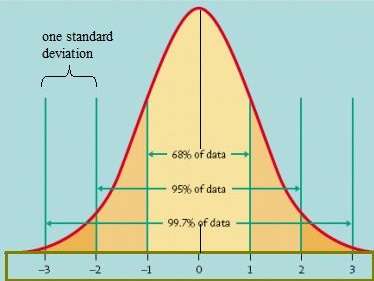
\includegraphics[width=5cm]{../../Graphs/68-95-99.jpg}
\end{center}
\tiny source: {\url http://www.statisticshowto.com/68-95-99-7-rule/}
\end{frame}
%%%%%%%%%%%%%%%%%%%%%%%%%%%%%
\begin{frame}
\frametitle{Certainty for linear regression}
Therefore,
$$
0.95 = P(L \leq y(x) \leq U) = P\left(\frac{L-f(x;\theta)}{\sigma} \leq e \leq \frac{U-f(x;\theta}{\sigma})\right).
$$
Using the normal distribution, we find that
$$
L-f(x;\theta) = -\sigma z_{1-\alpha/2}, \quad U-f(x;\theta) = \sigma z_{1-\alpha/2}.
$$
This gives 
$$
L = f(x;\theta) -\sigma z_{1-\alpha/2}, \quad U = f(x;\theta) + \sigma z_{1-\alpha/2}.
$$
For $\alpha=5\%$, this gives
$$
(L,U) = f(x;\theta) \pm 1.96 \sigma.
$$
\end{frame}
%%%%%%%%%%%%%%%%%%%%%%%%%%%%%
\begin{frame}
\frametitle{Certainty for linear regression}
Using a plug-in estimate, this gives us a {\it rough} prediction interval (at $95\%$) of
$$
(\hat{L},\hat{U}) = f(x;\hat{\theta}) \pm 1.96 s, 
$$
where $s$ is the unbiased estimate of the standard deviation
$$
s^2 = \frac{1}{n-(p+1)} \sum_{i=1}^n \{y_i - f(x_i;\hat{\theta})\}^2.
$$
This prediction interval is however hardly used/implemented because
\begin{itemize}
\item the estimate $s$ carries uncertainty. If taken into account, the Student $t_{n-(p+1)}$ distribution should be used.
\item the estimate $\hat{\theta}$ carries uncertainty. If taken into account, the estimate of $s$ should be changed to $s \sqrt{1+x^T(X^TX)^{-1}x}$.
\end{itemize}
Both adaptations widen the interval. 
\end{frame}
%%%%%%%%%%%%%%%%%%%%%%%%%%%%%
\begin{frame}
\frametitle{Certainty for logistic regression}
The probability provides an interpretation of the certainty the model provides on a classification. Consider: 
\begin{itemize}
\item $\hat{y}=1$ with $\hat{p} = 0.99$: the prediction is {\bf certain}.
\item $\hat{y}=1$ with $\hat{p} = 0.53$: the prediction is {\bf uncertain}.
\end{itemize}
In both cases, the predicted class is the same but the probability provides a more precise view on it: if the instance is far in the class or on the edge between the two classes.\\
\vspace{0.2cm}
The prediction "Good" for a customer with a probability of $0.51$ is uncertain. Alternatively, the prediction rule could set to a larger value than 0.5 to increase the certainty. \\
\vspace{0.2cm}
Also, a model with a lot of predictions close to 0.5 is of considered as poor because of its uncertainty\footnote{A little thought on that will brings us back to the entropy.}.
\end{frame}
%%%%%%%%%%%%%%%%%%%%%%%%%%%%%
\section{Selection of variables}
%%%%%%%%%%%%%%%%%%%%%%%%%%%%%
\begin{frame}
\frametitle{Occam's Razor}
A parsimony principle:
\begin{center}
"All else being equal, the simplest explanation is the best one"
\end{center}
\begin{itemize}
\item In other words, among two models with approximately the same prediction quality, choose the simplest one. 
\item In practice, we remove from the model variables that do not impair too much the prediction quality. 
\end{itemize}
Simplifying the model is a solution to {\bf overfitting}. This will be studied later in the course.
\end{frame}
%%%%%%%%%%%%%%%%%%%%%%%%%%%%%
\begin{frame}
\frametitle{Akaike Information Criterion}
The {\bf AIC} (Akaike Information Criterion) is 
$$
AIC = -2\hat{\ell} + 2k
$$
where 
\begin{itemize}
\item $\hat{\ell}$ is the maximum {\bf log-likelihood} and measure the goodness-of-fit, 
\item $k$ is the number of parameters and measure the model complexity.
\end{itemize}
{\bf Minimizing} the AIC achieves a trade-off between the quality of prediction and the model complexity.
\end{frame}
%%%%%%%%%%%%%%%%%%%%%%%%%%%%%
\begin{frame}
\frametitle{Akaike Information Criterion}
For linear regressions,
\begin{itemize}
\item The number of parameters is $k=p+2$ with $\theta_0,\theta_1,\ldots,\theta_p$ and $\sigma$,
\item The log-likelihood part equals
$$
-2\hat{\ell} = n\ln 2\pi + n \ln \hat{\sigma}^2 + \frac{1}{\hat{\sigma}^2}\sum_{i=1}^n \left\{y_i - f(x;\hat{\theta})\right\}^2,
$$
where $\hat{\sigma}^2 = (n-p-1)s^2/n$.
\end{itemize}
For logistic regressions,
\begin{itemize}
\item The number of parameters is $k=p+1$ for $\theta_0,\theta_1,\ldots,\theta_p$, 
\item The log-likelihood part equals
$$
-2\hat{\ell} = 2 \sum_{i=1}^n y_i \ln p(x_i;\hat{\theta}) + (1-y_i) \ln \{1-p(x_i;\hat{\theta})\}.
$$
\end{itemize}
\end{frame}
%%%%%%%%%%%%%%%%%%%%%%%%%%%%%
\begin{frame}
\frametitle{Variables selection with AIC}
Automatic variable selection using stepwise minimization of the AIC can be performed. There are 
\begin{itemize}
\item Backward: start from the most complete model and try to remove variable one at a time (if it decreases the AIC)
\item Forward: start from the empty model and try to add one variable at a time (if it decreases the AIC).
\item Both: start to add or remove at each step.
\end{itemize}
At each step, all the models in competition are fitted. The procedure is computationally intense.
\end{frame}
%%%%%%%%%%%%%%%%%%%%%%%%%%%%%
\begin{frame}
\frametitle{Variable selection with penalization}
A different approach consists of penalizing the loss function so that, during the training of the parameters, the variable selection applies directly.\\
\vspace{0.3cm}
The most common penalties are:
\begin{itemize}
\item $L_1$ penalty (LASSO)
$$
\min_\theta \bar{\cal L}(\theta) + \lambda \sum_{j=1}^p \vert \theta_j \vert
$$
\item $L_2$ penalty (Ridge)
$$
\displaystyle \min_\theta \bar{\cal L}(\theta) + \lambda \sum_{j=1}^p \theta_j^2
$$
\end{itemize} 
Usually, $\theta_0$ is not penalized. 
\end{frame}
%%%%%%%%%%%%%%%%%%%%%%%%%%%%%
\begin{frame}
\frametitle{Variable selection with penalization}
The penalty parameter $\lambda \geq 0$:
\begin{itemize}
\item If $\lambda =0$, then there is no penalty.
\item If $\lambda \longrightarrow \infty$, then $\theta \longrightarrow 0$.
\end{itemize}
For intermediate values, some components of $\theta$ will be small, pushed toward $0$.\\ \vspace{0.3cm}
This is equivalent to variable selection: setting $\theta_j=0$ is equivalent to not including $x_j$.\\
\vspace{0.3cm}
Selection of $\lambda$ can be done with cross-validation (see later).
\end{frame}
%%%%%%%%%%%%%%%%%%%%%%%%%%%%%
\begin{frame}
\frametitle{Variable selection with penalization}
\begin{itemize}
\item $L_1$ shrink some of the $\theta_j$, set some $\theta_j = 0$, select variables.
\item $L_2$ shrink all the $\theta_j$'s, avoiding extremes $\theta_j$, regularize $\theta$. 
\end{itemize}
{\bf Elastic net} combines $L_1$ and $L_2$:
$$
\displaystyle \min_\theta \bar{\cal L}(\theta) + \lambda \left\{\alpha \sum_{j=1}^p \vert \theta_j  \vert + \frac{1-\alpha}{2}\sum_{j=1}^p \theta_j^2\right\}
$$
with $0 \leq \alpha \leq 1$,
\begin{itemize}
\item If $\alpha=0$, it is the ridge ($L_2$)
\item If $\alpha=1$, it is the LASSO ($L_1$)
\end{itemize}
Often, $\lambda$ is selected by the data (cv), while $\alpha$ is set by the user.
\end{frame}
%%%%%%%%%%%%%%%%%%%%%%%%%%%%%
\end{document}


%%%%%%%%%%%%%%%%%%%%%%%%%%%%%
%%%%%%%%%%%%%%%%%%%%%%%%%%%%%
%%%%%%%%%%%%%%%%%%%%%%%%%%%%%
%% Old
\begin{frame}[fragile]
\frametitle{Variables selection}
The selection (backward direction) based on the AIC
\tiny
\begin{verbatim}
> step(fb3.lm)
Start:  AIC=6634.25
Lifetime.Post.Consumers ~ Page.total.likes + Type + Category + 
    Post.Month + Post.Weekday + Post.Hour + Paid

                   Df Sum of Sq       RSS    AIC
- Post.Weekday      6   4719414 271915846 6631.0
- Post.Hour         1    190145 267386576 6632.6
- Post.Month       11  11337076 278533507 6633.0
<none>                          267196431 6634.3
- Page.total.likes  1   2096407 269292838 6636.2
- Category          2   4023285 271219716 6637.7
- Paid              1   4370739 271567170 6640.3
- Type              3  81007578 348204009 6760.4

Step:  AIC=6630.99
Lifetime.Post.Consumers ~ Page.total.likes + Type + Category + 
    Post.Month + Post.Hour + Paid

                   Df Sum of Sq       RSS    AIC
- Post.Month       11  10836340 282752186 6628.5
- Post.Hour         1    289308 272205154 6629.5
<none>                          271915846 6631.0
- Page.total.likes  1   1860856 273776701 6632.4
- Category          2   3841983 275757829 6634.0
- Paid              1   3492554 275408400 6635.4
- Type              3  82511560 354427406 6757.2
\end{verbatim}
\end{frame}
%%%%%%%%%%%%%%%%%%%%%%%%%%%%%
\begin{frame}[fragile]
\frametitle{Variables selection}
\tiny
\begin{verbatim}
Step:  AIC=6628.49
Lifetime.Post.Consumers ~ Page.total.likes + Type + Category + 
    Post.Hour + Paid

                   Df Sum of Sq       RSS    AIC
- Post.Hour         1    256524 283008710 6626.9
<none>                          282752186 6628.5
- Category          2   2970606 285722792 6629.7
- Paid              1   3785863 286538049 6633.1
- Page.total.likes  1  24706505 307458691 6668.3
- Type              3  81149016 363901202 6748.4

Step:  AIC=6626.94
Lifetime.Post.Consumers ~ Page.total.likes + Type + Category + 
    Paid

                   Df Sum of Sq       RSS    AIC
<none>                          283008710 6626.9
- Category          2   2771726 285780435 6627.8
- Paid              1   3978146 286986856 6631.9
- Page.total.likes  1  24512812 307521522 6666.4
- Type              3  80920617 363929327 6746.4

\end{verbatim}
\end{frame}
%%%%%%%%%%%%%%%%%%%%%%%%%%%%%
\begin{frame}[fragile]
\frametitle{Variables selection}
The final model is
\tiny
\begin{verbatim}
Call:
lm(formula = Lifetime.Post.Consumers ~ Page.total.likes + Type + 
    Category + Paid, data = facebook.dat)

Coefficients:
     (Intercept)  Page.total.likes         TypePhoto  
       1903.6819           -0.0142          554.8457  
      TypeStatus         TypeVideo        CategoryC2  
       1989.8878         1484.3815         -105.0015  
      CategoryC3           PaidYes  
       -179.4245          199.5205
\end{verbatim}
\normalsize
It removes first {\tt Post.Weekday} then {\tt Post.Month} then {\tt Post.Hour} then the best choice is {\tt <none>}.
\end{frame}
%%%%%%%%%%%%%%%%%%%%%%%%%%%%%


\begin{frame}[fragile]
\frametitle{Model assumptions}
A commonly used (unbiased) estimate of $\sigma^2$ is\footnote{for short we write $y(x_i;\hat{a})=\hat{y}_i$.} 
$$
s^2 = \frac{1}{n-(p+1)} \sum_{i=1}^n (y_i-\hat{y}_i)^2
$$
{\bf Example}: $s$ was estimated at $751.6$.\\
\scriptsize
\begin{verbatim}
> summary(fb3.lm)
[...]
Residual standard error: 751.6 on 473 degrees of freedom
[...]
\end{verbatim}
\end{frame}
%%%%%%%%%%%%%%%%%%%%%%%%%%%%%
\begin{frame}
\frametitle{Model assumptions}
Are model assumptions important? Yes and No.
\begin{itemize}
\item Yes if you use linear regression in a statistical approach (inference, tests, ANOVA, etc.). Then the p-values are computed {\it under the normal residual assumption} and are correct only if the model validate them.
\item No if you use it as a ``black box'' learner. The ML approach will judge the linear regression with a score computed on the test set (or through CV/bootstrap) solely based on the predictions. Even if the normal assumption is not valid, a good predictor is a good predictor.
\end{itemize}
\end{frame}
%%%%%%%%%%%%%%%%%%%%%%%%%%%%%
\begin{frame}
\frametitle{Coefficients and weights}
The previous graph represents the linear regression as a neural network (a very simple one).
\begin{itemize}
\item The coefficients $a_0, a_1, \ldots, a_p$ are also called the {\bf weights} of the model (NN). 
\item The coefficient $a_0$ is called the {\bf intercept} (linear model) or the {\bf bias} (NN)
\item The $p+1$ coefficient $a=(a_0,\ldots,a_p)$ are estimated during the training of the model.\\
\item All the features in $x$ are numerical; in particular, all categorical variables are interpreted through their dummy variables. 
\end{itemize}
\end{frame}
%%%%%%%%%%%%%%%%%%%%%%%%%%%%%
\begin{frame}
\frametitle{The residuals}
The {\bf residual} for the instance $i$ is the difference between the observed $y_i$ and the predicted one $y(x_i;a)$ (syn. the {\bf error}):
$$
e_i = y_i - y(x_i;a).
$$
\end{frame}
%%%%%%%%%%%%%%%%%%%%%%%%%%%%%
\begin{frame}
\frametitle{Estimation}
Usually, during the training, the estimation of $a$ is obtained by the minimization of the {\bf sum-of-squares}
\begin{eqnarray*}
SS(a) &=& \sum_{i=1}^n \left(y_i - y(x_i;a)\right)^2 \\
&=& \sum_{i=1}^n \left\{y_i - (a_0 + a_1 x_{1i} + \ldots + a_p x_{pi})\right\}^2\\
&=& \sum_{i=1}^n e_i^2
\end{eqnarray*}
A model with a small $SS(\hat{a})$ achieves a good match between the predictions and the observations. The {\bf ordinary least square} estimate (OLS) is
$$
\hat{a} = \arg\min_a SS(a).
$$
\end{frame}
%%%%%%%%%%%%%%%%%%%%%%%%%%%%%
\begin{frame}
\frametitle{Example}
A study aims to predict the performance metrics of posts published
in brands' Facebook pages. In the original paper\footnote{(Moro et al., 2016) Moro, S., Rita, P., $\&$ Vala, B. (2016). Predicting social media performance metrics and evaluation of the impact on brand building: A data mining approach. Journal of Business Research, 69(9), 3341-3351.}, twelve posts' performance metrics extracted from a cosmetic company's page including 790 publications were modeled to understand how each of the seven input features influenced it. \\
\vspace{0.2cm}
Below, we focus on the numerical outcome {\tt Lifetime Post Consumers} to illustrate the method. We only have access to 500 posts (instances).
\end{frame}
%%%%%%%%%%%%%%%%%%%%%%%%%%%%%
\begin{frame}
\frametitle{Example}
\begin{itemize}
\item Outcome $y$: {\tt Lifetime Post Consumers} - the number of people who clicked anywhere in a post.
\item The seven features are 
\begin{itemize}
\scriptsize
\item $x_1$: {\tt Page.total.likes} Number of people who have liked the company's page (!!page $\neq$ post).
\item $x_2$: {\tt Type} Type of content (Link, Photo, Status, Video)
\item $x_3$: {\tt Category} Manual content characterization (C1, C2, C3): action (special offers and
contests), product (direct advertisement, explicit brand content), and inspiration (non-explicit brand related content).
\item $x_4$: {\tt Post.Month} Month the post was published (January, February, March, ...,
December).
\item $x_5$: {\tt Post.Weekday} Weekday the post was published (Sunday, Monday, ...,
Saturday)
\item $x_6$: {\tt Post.Hour} Hour the post was published (0, 1, 2, 3, 4, ..., 23).
\item $x_7$: {\tt Paid} If the company paid to Facebook for advertising (yes, no).
\end{itemize}
\item There are 500 instances.
\end{itemize}
\end{frame}
%%%%%%%%%%%%%%%%%%%%%%%%%%%%%
\begin{frame}[fragile]
\frametitle{Example}
With the two features {\tt Page.total.likes} $(x_1)$ and {\tt Paid} $(x_7)$\\ 
\scriptsize
\begin{verbatim}
Coefficients:
     (Intercept)  Page.total.likes           PaidYes  
      1734.52147          -0.00801         186.77882   
\end{verbatim}
\normalsize
In this case,
$$
y(x;\hat{a}) = 1734.5 - 0.008 x_1 + 186.8 x_7,
$$
where $x_7 = 1$ if {\tt Paid = Yes}, and 0 if {\tt Paid = No}. We have
$$
\hat{a}_0 = 1734.5, \quad \hat{a}_1=-0.008, \hat{a}_7=186.6.
$$
Looking at the first instance $i=1$, we have
\begin{center}
\begin{tabular}{|c|c|c|c|c|c|c|}
\hline
$y_1$ & $x_{11}$ & $x_{17}$ & $\hat{y}_1$ & $e_1$\\
\hline
109 & 139441 & 0 & 617.5 & -508.5\\
\hline
\end{tabular}
\end{center}
\end{frame}
%%%%%%%%%%%%%%%%%%%%%%%%%%%%%
\begin{frame}[fragile]
\frametitle{Example}
When adding {\tt Category} to the model gives\\ 
\scriptsize
\begin{verbatim}
Coefficients:
     (Intercept)  Page.total.likes        CategoryC2  
      1968.68322          -0.01022         288.64808  
      CategoryC3           PaidYes  
      -128.47698         195.95560
\end{verbatim}
\normalsize
The prediction equation is
$$
y(x;\hat{a}) = 1968.7 - 0.010 x_1 + 288.6 x_{3,1} - 28.5 x_{3,2}+ 196.0 x_7.
$$
\end{frame}
%%%%%%%%%%%%%%%%%%%%%%%%%%%%%
\begin{frame}[fragile]
\frametitle{Example}
{\bf Example}: Extending this with all the available features gives\\ 
\tiny
\begin{verbatim}
Coefficients:
     (Intercept)  Page.total.likes         TypePhoto  
       5348.8727           -0.0463          534.9196  
      TypeStatus         TypeVideo        CategoryC2  
       1993.5764         1527.9009         -194.5406  
      CategoryC3     Post.MonthAug     Post.MonthDec  
       -227.0303          795.2857         1034.8361  
   Post.MonthFeb     Post.MonthJan     Post.MonthJul  
       -201.2036         -777.4440          895.1965  
   Post.MonthJun     Post.MonthMar     Post.MonthMay  
        727.4582         -338.0111          281.9842  
   Post.MonthNov     Post.MonthOct     Post.MonthSep  
        675.2298         1016.5307          988.2724  
 Post.WeekdayMon   Post.WeekdaySat   Post.WeekdaySun  
        239.8912           34.8302           55.8315  
 Post.WeekdayThu   Post.WeekdayTue   Post.WeekdayWed  
        -26.9925            6.8544          223.9480  
       Post.Hour           PaidYes  
         -4.8014          216.0266 
\end{verbatim}
\normalsize
\end{frame}
%%%%%%%%%%%%%%%%%%%%%%%%%%%%%
\begin{frame}
\frametitle{Interpretation of the coefficients}
One appealing aspect of linear models is the interpretability of their coefficients. They are interpreted as {\it slopes}.
\begin{itemize}
\item When the feature $x_1$ increases by $1$ unit, the outcome $y$ increases in average by $a_1$ units (same for all features $1,\ldots,p$).
\item A positive weight $a_j$ means a positive linear association between the feature $x_j$ and the outcome $y$.
\item The larger the coefficients, the larger the association, in absolute value. (note: pay attention to the scale!)
\item For the categorical features, the coefficients estimate the average change in the outcome $y$ when the feature switches from the reference level to any other level. It is thus a {\bf contrast} with the reference level.  
\end{itemize}
\end{frame}
%%%%%%%%%%%%%%%%%%%%%%%%%%%%%
\begin{frame}
\frametitle{Example}
Case with {\tt Page.total.likes}, {\tt Category}, {\tt Paid}:
\begin{itemize}
\item If {\tt Page.total.likes} increases by 1 unit, then {\tt Lifetime.Post.Consumers} decreases in average by $(-)0.01$ units.
\item Switching {\tt Paid} from {\tt No} to {\tt Yes}, increases in average by 196 units.
\item Switching {\tt Category} from {\tt C1} to {\tt C2} increases in average the outcome by 288.6. 
\item Switching {\tt Category} from {\tt C1} to {\tt C3} decreases in average the outcome by $(-)128.5$. 
\end{itemize}
\end{frame}
%%%%%%%%%%%%%%%%%%%%%%%%%%%%%
\begin{frame}
\frametitle{Model assumptions}
It is often assumed that the residuals $e_i$ are independent and normally distributed with a standard deviation $\sigma$:
$$
e_i \stackrel{i.i.d}{\sim} N(0, \sigma^2).
$$
In particular, we expect the residual distribution to be symmetric around $0$ and (informally) respect the 68-95-99.7 rule:
\begin{center}
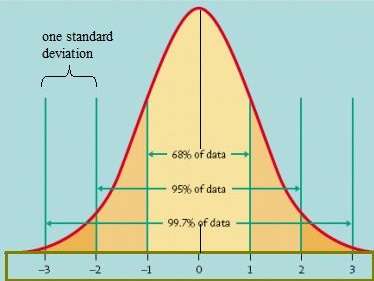
\includegraphics[width=5cm]{../../Graphs/68-95-99.jpg}
\end{center}
\tiny source: {\url http://www.statisticshowto.com/68-95-99-7-rule/}
\end{frame}
%%%%%%%%%%%%%%%%%%%%%%%%%%%%%
\begin{frame}[fragile]
\frametitle{Model assumptions}
A commonly used (unbiased) estimate of $\sigma^2$ is\footnote{for short we write $y(x_i;\hat{a})=\hat{y}_i$.} 
$$
s^2 = \frac{1}{n-(p+1)} \sum_{i=1}^n (y_i-\hat{y}_i)^2
$$
{\bf Example}: $s$ was estimated at $751.6$.\\
\scriptsize
\begin{verbatim}
> summary(fb3.lm)
[...]
Residual standard error: 751.6 on 473 degrees of freedom
[...]
\end{verbatim}
\end{frame}
%%%%%%%%%%%%%%%%%%%%%%%%%%%%%
\begin{frame}
\frametitle{Model assumptions}
Are model assumptions important? Yes and No.
\begin{itemize}
\item Yes if you use linear regression in a statistical approach (inference, tests, ANOVA, etc.). Then the p-values are computed {\it under the normal residual assumption} and are correct only if the model validate them.
\item No if you use it as a ``black box'' learner. The ML approach will judge the linear regression with a score computed on the test set (or through CV/bootstrap) solely based on the predictions. Even if the normal assumption is not valid, a good predictor is a good predictor.
\end{itemize}
\end{frame}
%%%%%%%%%%%%%%%%%%%%%%%%%%%%%
\section{Logistic regression}
%%%%%%%%%%%%%%%%%%%%%%%%%%%%%
\begin{frame}
\frametitle{Logistic regression}
The logistic regression is a regression adapted to binary classification. The linear combination is transformed to a probability using a {\bf sigmoid function}.\\
\vspace{0.2cm}
The {\bf linear predictor}:
$$
z_i = a_0 + a_1 x_{1i} + \cdots + a_p x_{pi},
$$
The {\bf probability prediction} (sigmoid):
$$
p_i = P(Y_i=1 | X_i=x_i) = \frac{\exp\{z_i\}}{1+\exp\{z_i\}}.
$$
The {\bf prediction of the class}: 
$$
y_i = \left\{
\begin{array}{ll}
1, & \mbox{if } p_i\geq 0.5,\\
0, & \mbox{if } p_i<0.5.
\end{array}
\right.
$$
\end{frame}
%%%%%%%%%%%%%%%%%%%%%%%%%%%%%
\begin{frame}
\frametitle{The logit function}
The {\bf logit function} is the inverse of the {\bf sigmoid function} and thus transforms $p_i$ to $z_i$.
$$
z_i = \log \frac{p_i}{1-p_i}
$$ 
Representation of a logistic regression:
\begin{center}
\includegraphics[width=5cm]{../../Graphs/LogReg_Network.png}
\end{center}
\end{frame}
%%%%%%%%%%%%%%%%%%%%%%%%%%%%%
\begin{frame}
\frametitle{Estimation}
The coefficients (or weights) are obtained by maximizing the {\bf log-likelihood}
$$
\ell(a) = \sum_{i=1}^n y_i \log p_i + (1-y_i) \log(1-p_i).
$$
This is equivalent to minimize the {\bf entropy}, which is the negative log-likelihood:
$$
E(a) = -\sum_{i=1}^n y_i \log p_i + (1-y_i) \log(1-p_i).
$$
\small
Notes: 
\begin{itemize}
\item the likelihood is more common to statistics, wherase entropy is more common to neural networks. They are however equivalent in this case. 
\item The entropy is sometimes expressed in $\log_2$.
\end{itemize}
\end{frame}
%%%%%%%%%%%%%%%%%%%%%%%%%%%%%
\begin{frame}
\frametitle{Interpretation}
Looking carefully, the log-likelihood sum up all the $\log p_i$ for which $y_i=1$ and all the $\log 1-p_i$ for which $y_i=0$:
$$
\ell(a) = \sum_i \log P(\mbox{observe }Y_i=y_i).
$$
In other words, this is the sum of the (log-)probabilities of observing what was actually observed.\\ 
\vspace{0.2cm}
Therefore, maximizing $\ell(a)$ is equivalent to look for a logistic regression that has the highest probability of observing what was indeed observed. And this makes sense...
\end{frame}
%%%%%%%%%%%%%%%%%%%%%%%%%%%%%
\begin{frame}
\frametitle{Interpretation of the coefficients}
Because of the sigmoid transform, the interpretation of the coefficients is more difficult than with the linear regression:
\begin{itemize}
\item With a positive $a_j$, an increase of $x_j$ is associated with an increase of the probability of $y=1$. 
\item The larger the coefficient, the larger the increase. However, it the increase is not linear and depends on the other features.
\item A negative coefficient means a decrease in the probability of the positive class ($y=1$).
\end{itemize}
\small
Note: one should not say that an increase in $x_j$ {\it causes} an increase of the probability. It is only an association. The causality implies a direction and is more complex to establish.
\normalsize
\end{frame}
%%%%%%%%%%%%%%%%%%%%%%%%%%%%%
\begin{frame}
\frametitle{Example}
A researcher studies how GRE (Graduate Record Exam scores), GPA (grade point average) and prestige of the undergraduate institution effects admission into graduate school (admit/don't admit).\footnote{source: {\url https://stats.idre.ucla.edu/r/dae/logit-regression/}}
\\
\vspace{0.3cm}
Variable {\tt rank} is categorical and represents the prestige institution prestige (1="High prestige" to 4="Low prestige"). {\tt rank} 1 is the reference level. 
\end{frame}
%%%%%%%%%%%%%%%%%%%%%%%%%%%%%
\begin{frame}[fragile]
\frametitle{Example}
\scriptsize
\begin{verbatim}
> mylogit <- glm(admit ~ gre + gpa + rank, data = mydata, family = "binomial")
> summary(mylogit)
[...]
Coefficients:
             Estimate Std. Error z value Pr(>|z|)    
(Intercept) -3.989979   1.139951  -3.500 0.000465 ***
gre          0.002264   0.001094   2.070 0.038465 *  
gpa          0.804038   0.331819   2.423 0.015388 *  
rank2       -0.675443   0.316490  -2.134 0.032829 *  
rank3       -1.340204   0.345306  -3.881 0.000104 ***
rank4       -1.551464   0.417832  -3.713 0.000205 ***
---
[...]
\end{verbatim}
\normalsize
\end{frame}
%%%%%%%%%%%%%%%%%%%%%%%%%%%%%
\begin{frame}
\frametitle{Example}
The interpretation of the coefficients are:
\begin{itemize}
\item {\tt gre} is positively associated with admission ($y=1$)
\item {\tt gpa} is also\footnote{An increase of 1 unit of {\tt gpa} is associated with a larger increase in the probability of being admitted than with an increase of 1 unit of {\tt gre}.} 
\item The predicted probability of being admitted for rank 2 is lower than for {\tt rank} 1.
\item The predicted probability of being admitted for rank 3 is lower than for {\tt rank} 1 (and also than lower for {\tt rank} 2).
\item etc.
\end{itemize}
\end{frame}
%%%%%%%%%%%%%%%%%%%%%%%%%%%%%
\begin{frame}
\frametitle{Example}
The prediction for {\tt gre}: 380, {\tt gpa}: 3.61, {\tt rank} 3 is
$$
z = -4.0 + 0.0023\times 380 + 0.80\times 3.61 - 1.34 = -1.578
$$
then
$$
p = \frac{e^{-1.578}}{1+e^{-1.578}} = 0.171 < 0.5
$$
then $\hat{y}=0$.\\ 
\vspace{0.2cm}
Note that the actual observation for this instance was indeed $y=0$. The contribution to the entropy of observation is thus\footnote{$0.27$ with $\log_2$}:
$$
-\log(1-0.171) = 0.081
$$
\end{frame}
%%%%%%%%%%%%%%%%%%%%%%%%%%%%%
\begin{frame}
\frametitle{Certainty}
The probability provides an interpretation of the certainty the model provides on a classification. Consider: 
\begin{itemize}
\item $\hat{y}=1$ with $\hat{p} = 0.99$: the prediction is {\bf certain}.
\item $\hat{y}=1$ with $\hat{p} = 0.53$: the prediction is {\bf uncertain}.
\end{itemize}
In both cases, the predicted class is the same but the probability provides a more precise view on it: if the instance is far in the class or on the edge between the two classes.\\
\vspace{0.2cm}
The prediction "Good" for a customer with a probability of $0.51$ is uncertain. Alternatively, the prediction rule could set to a larger value than 0.5 to increase the certainty. \\
\vspace{0.2cm}
Also, a model with a lot of predictions close to 0.5 is of considered as poor because of its uncertainty\footnote{A little thought on that will brings us back to the entropy.}.
\end{frame}
%%%%%%%%%%%%%%%%%%%%%%%%%%%%%
\end{document}

